% !TeX encoding = UTF-8
% !TeX spellcheck = en_GB
% !TeX root = ../Thesis_AndreGuerra.tex
%%%%%%%%%%%%%%% Thesis_InstitutionsFunding.tex %%%%%%%%%%%%%%
%
% PhD thesis - Institutions Involved and Funding
% André Guerra
%
% 18/Apr/2017
%
%%%%%%%%%%%%%%%%%%%%%%%%%%%%%%%%%%%%%%%%%%%%%%%%%%%%%%%%%%%%%


\newpage{
    \thispagestyle{empty}
    
    \Large{Institutions where the work was carried out:}
    
    \vskip 1cm
    
    \capstartfalse
    \begin{figure}[h!]
        \centering
        \begin{subfigure}[c]{0.45\textwidth}
            \centering
            
\includegraphics[width=0.9\textwidth]{FCUP_eps}
        \end{subfigure}
        \hfill %add desired spacing between images, e. g. ~, \quad, \qquad, \hfill etc. 
          %(or a blank line to force the subfigure onto a new line)
        \begin{subfigure}[c]{0.45\textwidth}
            \centering
            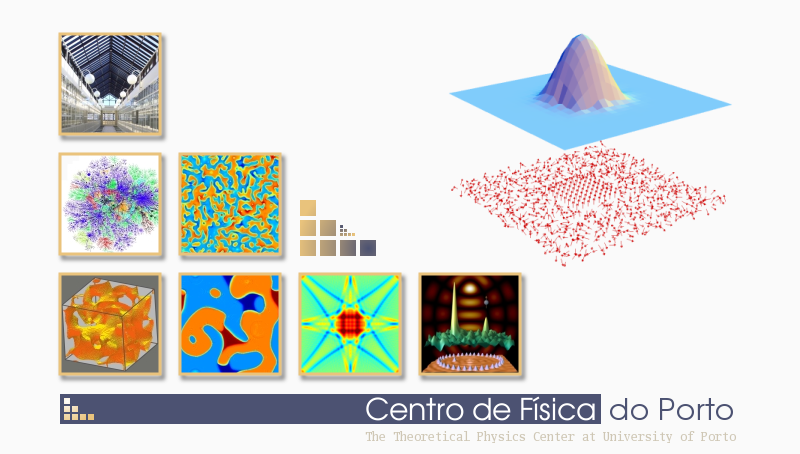
\includegraphics[width=0.7\textwidth]{CFP}
        \end{subfigure}
        
        \vspace*{0.4cm}
        
        \begin{subfigure}[c]{0.45\textwidth}
            \centering
            
\includegraphics[width=0.4\textwidth]{LSTS}
        \end{subfigure}
        \hfill %add desired spacing between images, e. g. ~, \quad, \qquad, \hfill etc. 
          %(or a blank line to force the subfigure onto a new line)
        \begin{subfigure}[c]{0.45\textwidth}
            \centering
            
\includegraphics[width=0.8\textwidth]{UVigo}
        \end{subfigure}
    \end{figure}
    
    \vskip 2cm

    \Large{Funding:}
    
    My PhD work was supported by the Funda{\c c}\~ao para a Ci\^encia e a Tecnologia (Portuguese Agency for Research) fellowship PD/BD/XXXXXX/XXXX.
    
    \vskip 1cm
    
    \begin{figure}[h!]
        \centering
        
\includegraphics[width=0.5\linewidth]{FCT}
        \caption*{}
    \end{figure}
    
    \vfill
}

% end of file Thesis_InstitutionsFunding.tex
%%%%%%%%%%%%%%%%%%%%%%%%%%%%%%%%%%%%%%%%%%%%%%%%%%%%%%%%%%%%%%%%%%%